\thispagestyle{empty}
\section{Praktische Durchführung}
\subsection{Hardware}
\subsection{Docker}
\subsection{Realisierung}
Im Linux-File-System ist es möglich cgroups über PID's ausfindig zu machen und die verwendeten Ressourcen auszugeben. Was mich auf die Idee brachte, einen neuen Docker-Container zu erstellen, in diesem einen Prozess mit einem einfachen malloc() befehlt in einer Endlosschleife auszuführen und die menge des allokierten Speichers der cgroup auszugeben. 

\subparagraph{Test01}
Über das online user interface war es einfach einen Docker-Container schnell zu erstellen. Ressourcen Limits konnten ebenfalls vor dem starten des Containers eingestellt werden. Für den ersten Start des Containers benötigen wir allerdings noch keine Begrenzung des Speichers, da es in erster Linie um die Auswirkung des ausgeführten C-Programms auf die eigene cgroup geht. Der verwendete C-Code den der Prozess ausführen wird, ist in Listing \ref{01mem} zu sehen. Ein selbst erstelltes Skript verwendet die beim Start erzeugte PID, findet die Cgroup in der der Prozess ausgeführt wird und schreibt die ausgelesenen Messdaten in ein txt-File. Die Messdaten wie Clock-Time in Nanosekunden und Speicherverbrauch in Bytes werden für die Auswertung verwendet.

\vspace{1em}
\lstinputlisting[caption=einfacher C-Code, label=01mem, basicstyle=\ttfamily\scriptsize]{code/01mem.txt}

\subparagraph{Erwartungshaltung Test 01}
Falls das Skript die Messwerte in ungefähr gleichmäßig schnellen Abständen liefert, und die Speicher Allocationen gleich schnell ablaufen, erwarte ich eine Gerade Funktion, die gleichbleibend schnell ansteigt und irgendwann wenn nicht mehr genug Speicher im System vorhanden ist beendet wird.

\vspace{1em}
\begin{minipage}{\linewidth}
	\centering
	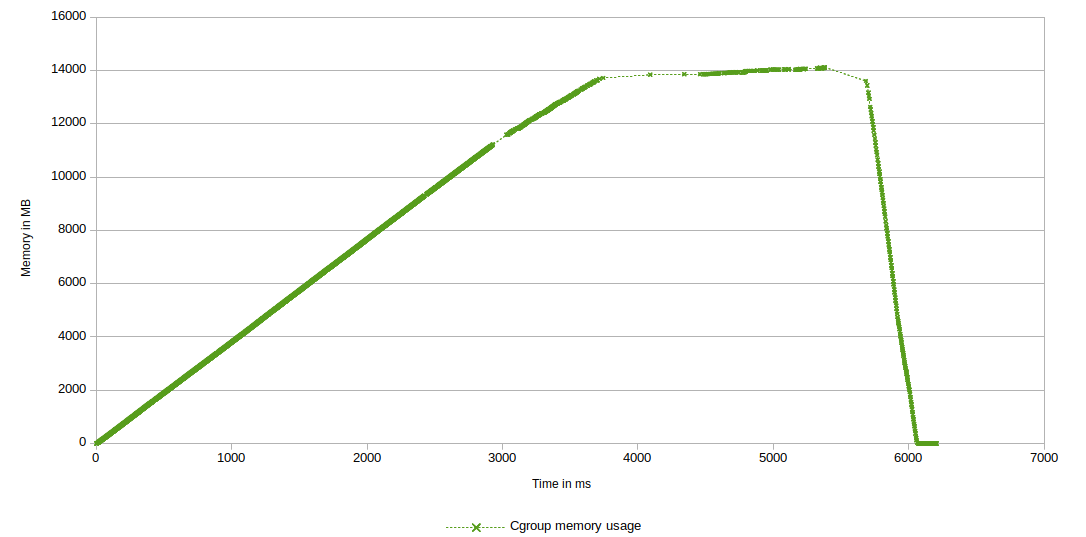
\includegraphics[width=1\linewidth]{pics/001_mem_usage_No_Limit_Cgroup_RDY_FOR_USE.png}
	\captionof{figure}[Speicher Verbrauch Cgroup Ohne Limit]{Memory usage Cgroup no Limit}
	\label{fig:001_mem_usage_No_Limit_Cgroup_RDY_FOR_USE}
\end{minipage}

\subparagraph{Ergebnis Test01}
In Abbildung \ref{fig:001_mem_usage_No_Limit_Cgroup_RDY_FOR_USE} ist wie erwartet eine gleichmäßige Steigung erkennbar. Bei ca. 13900MB Allociertem Speicher bricht die Wachstumsrate zusammen. An diesem Punkt ist der insgesamt 16GB große Arbeitsspeicher offenbar größtenteils Ausgeschöpft. Ein paar MB konnten vom Betriebssystem für den dauerhaft nach mehr Speicher verlangendem Prozess bereitgestellt werden. Bei knapp über 14000MB wurde der OOM-Killer eingeschaltet um wichtigere Prozesse zu schützen, und unser Container wurde beendet.

\subparagraph{Test02}
Im nächsten Schritt wäre es interessant zu sehen wie der Graph der Cgroup verläuft, wenn man ein Speicherlimit festlegt, das nicht überschritten werden soll (Hard-Limit). Um dieses Limit zu erstellen, wurde im User-Interface  das Ressourcenlimit auf 8200 Megabyte gesetzt und das in Listing \ref{01mem} vorgestellte Programm nochmals ausgeführt.

\subparagraph{Erwartungshaltung Test 02}
Da nun ein Hard-Limit gesetzt wurde kann ich mir vorstellen, dass die Cgroup mit der gleichen Geschwindigkeit wie in Abbildung \ref{fig:001_mem_usage_No_Limit_Cgroup_RDY_FOR_USE} bis zum gesetzten Limit ansteigt und dieses nicht überschreitet. 

\vspace{1em}
\begin{minipage}{\linewidth}
	\centering
	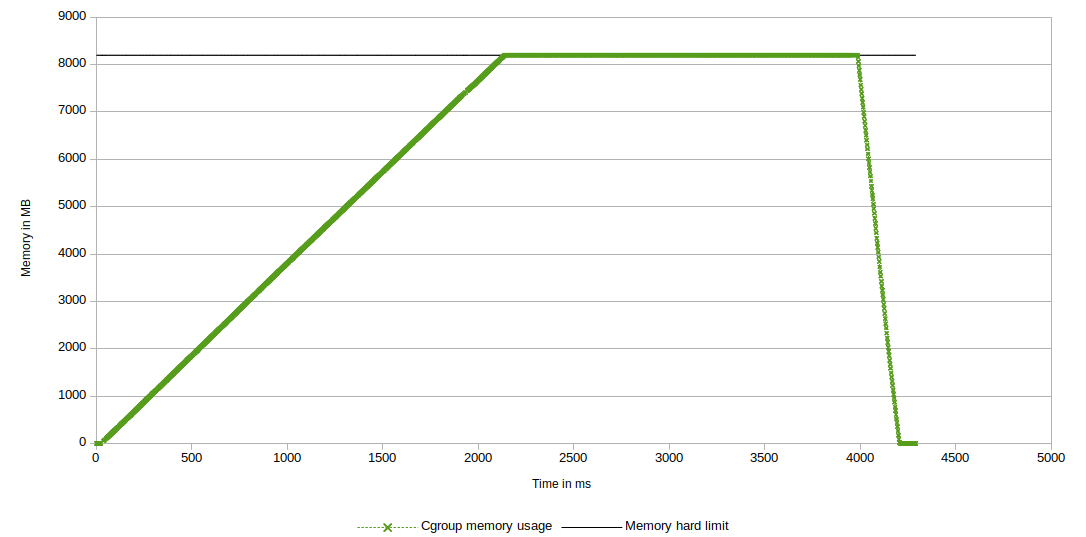
\includegraphics[width=1\linewidth]{pics/002_mem_usage_8200mb_limit_Cgroup_RDY_FOR_USE.png}
	\captionof{figure}[Speicher Verbrauch Cgroup 8200MB Limit]{Memory usage Cgroup 8200MB Limit}
	\label{fig:002_mem_usage_8200mb_limit_Cgroup_RDY_FOR_USE}
\end{minipage}

\subparagraph{Ergebnis Test02}
Mit einer Allocations Rate von ca. 4000MB/S ändert sich an der Speicher Zugriffsrate nichts, das Limit von 8200MB wurde erfolgreich eingehalten und der Prozess wurde wieder vom System beendet.

Schon fast Vorbildlich hält sich die Cgroup an das gesetzte Limit. Da frag ich mich "wie kann ich mir eine Cgroup vorstellen, was zeigt sie mir an, wie weit kann sie verwendete Ressourcen der einzelnen Prozesse verfolgen?". 

Meine Vorstellung einer Cgroup:
Die Cgroup ist wie eine Box. Die Größe der Box wird bei der Erstellung des Containers festgelegt. In unserem Fall sind das 8200MB. Der Füllstand der Box setzt sich aus den verwendeten Ressourcen aller in der Box ausgeführten Prozesse zusammen. Wenn ein Prozess nun wie in Abbildung \ref{fig:002_mem_usage_8200mb_limit_Cgroup_RDY_FOR_USE} die Komplette Box ausfüllt und weiter darüber hinaus ragen würde, wäre meine Box nur in der Lage den Füllstand bis zu Ihrer Maximalgröße von 8200 MB wiederzuspiegeln.

\subparagraph{Test03}
Nach meiner Vorstellung der Anzeigemöglichkeiten einer Cgroup liegt es nun nahe, sich den Prozess der durch das Ausführen des oben genannten C-Codes entsteht, selbst genauer anzusehen. Der Test02 wird mit einer Skript Erweiterung um die Anzahl der verwendeten Memory-Pages des Prozesses wiederholt. Eine Memory-Page ist 4KB groß und wird für die Auswertung mit der Anzahl an Memory-Pages multipliziert.

\subparagraph{Erwartungshaltung Test 03}
Wenn die Memory-Page Größe multipliziert mit der Anzahl an verwendeten Memory-Pages genau dem entspricht, was die Cgroup an Speicher Allocation ausgibt, sollten beide Graphen bis zum erreichen des Limits parallel verlaufen.

\vspace{1em}
\begin{minipage}{\linewidth}
	\centering
	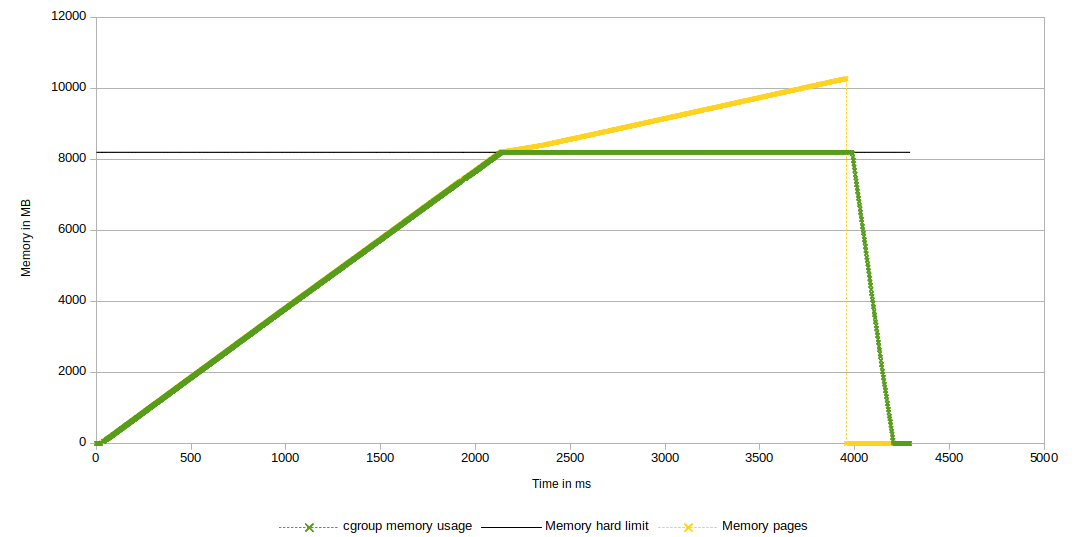
\includegraphics[width=1\linewidth]{pics/003_mem_usage_8200mb_limit_Cgroup_Pages_RDY_FOR_USE.png}
	\captionof{figure}[Speicher Verbrauch Cgroup 8200MB Limit]{Memory usage Cgroup 8200MB Limit}
	\label{fig:003_mem_usage_8200mb_limit_Cgroup_Pages_RDY_FOR_USE}
\end{minipage}

\subparagraph{Ergebnis Test03}
Deutlich zu erkennen sind die exat aufeinanderliegeneden Messwerte der Cgroup und der Memory Pages. Ab 8200MB schießen die allocierten Memory Pages bis ca 10200MB über das Limit hinaus. Erkennbar ist auch die geringere Allocationsrate von ca. 2000MB/s. Komplett ignoriert wurde das Limit allerdings nicht. Verglichen mit Test01 war noch genügend Speicher im System vorhanden. Wieso wurde der Prozess dann überhaupt schon beendet, warum konnte er über das Limit hinaus allokieren, wie verhält sich mein Container wenn ich nur ein bisschen über meinem Limit bin, wie wirkt sich das auf andere Container im System aus?

\subparagraph{Test04}
Um auf die aufgekommenen Fragen in Paragraph "Ergebnis Test03" hin zu arbeiten, benötigen wir nun einen Container der für eine gewisse Zeitspanne läuft und etwas mehr als das gesetzte Limit allociert. Der in Listing \ref{01mem} gezeigte C-Code wurde zu Listing \ref{02mem} verändert. 

\vspace{1em}
\lstinputlisting[caption=einfacher C-Code, label=02mem, basicstyle=\ttfamily\scriptsize]{code/02mem.txt}

\subparagraph{Erwartungshaltung Test 04}
Nachdem der Malloc(sizeof(int)*1024) befehl nun 2200001 mal ausgeführt wird, ein Integer 4Byte groß ist *1024 sind 4KB pro ausführung, sollte der Graph der Memory Pages bei etwa 8600MB verharren und 60 Sekunden diesen Wert halten.

\vspace{1em}
\begin{minipage}{\linewidth}
	\centering
	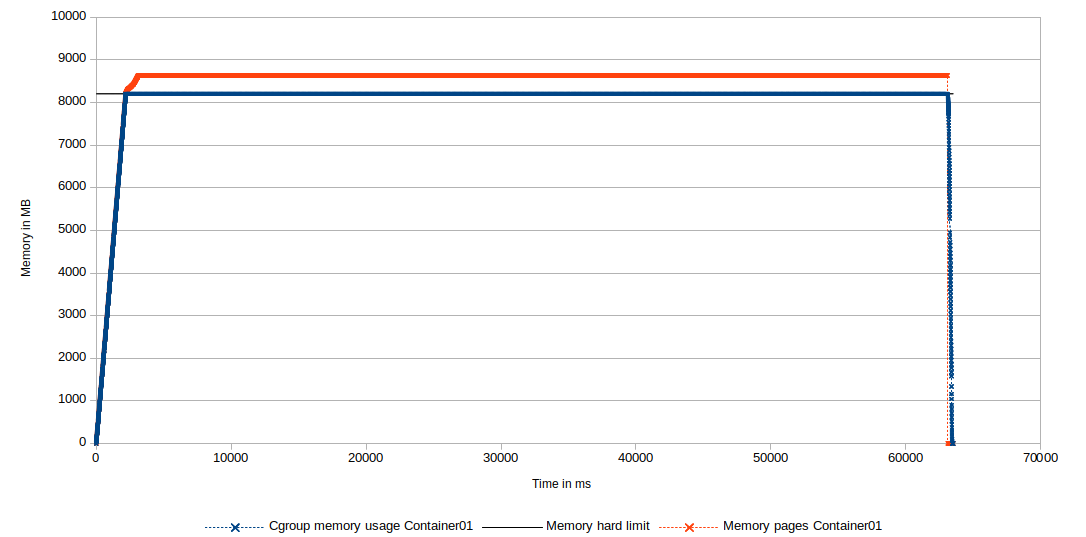
\includegraphics[width=1\linewidth]{pics/004_mem_usage_8200mb_limit_Container01_Basis_RDY_FOR_USE.png}
	\captionof{figure}[Speicher Verbrauch Cgroup 8200MB Limit]{Memory usage Cgroup 8200MB Limit}
	\label{fig:004_mem_usage_8200mb_limit_Container01_Basis_RDY_FOR_USE}
\end{minipage}

\subparagraph{Ergebnis Test04}
Wie man aus Abbildung \ref{fig:004_mem_usage_8200mb_limit_Container01_Basis_RDY_FOR_USE} entnehmen kann, ist es möglich für einen längeren Zeitraum über das Limit hinaus Ressourcen zu Allokieren. Durch die lange Ausführungszeit gleichbleibender Ressourcen ist es gut möglich den Einfluss von Container untereinander zu untersuchen. Diesen Container nenne ich von nun an Container01.

\subparagraph{Test05}
Im Ablauf des folgenden Tests wird zuerst Container01 gestartet, und während der Laufzeit wird Container02 ebenfalls eingeschaltet. Den Container02 habe ich zum besseren Verständnis in Abbildung \ref{fig:005_mem_usage_8200mb_limit_Container02_Basis_RDY_FOR_USE_FOCUS} nochmals in skalierter Umgebung dargestellt. 


\vspace{1em}
\begin{minipage}{\linewidth}
	\centering
	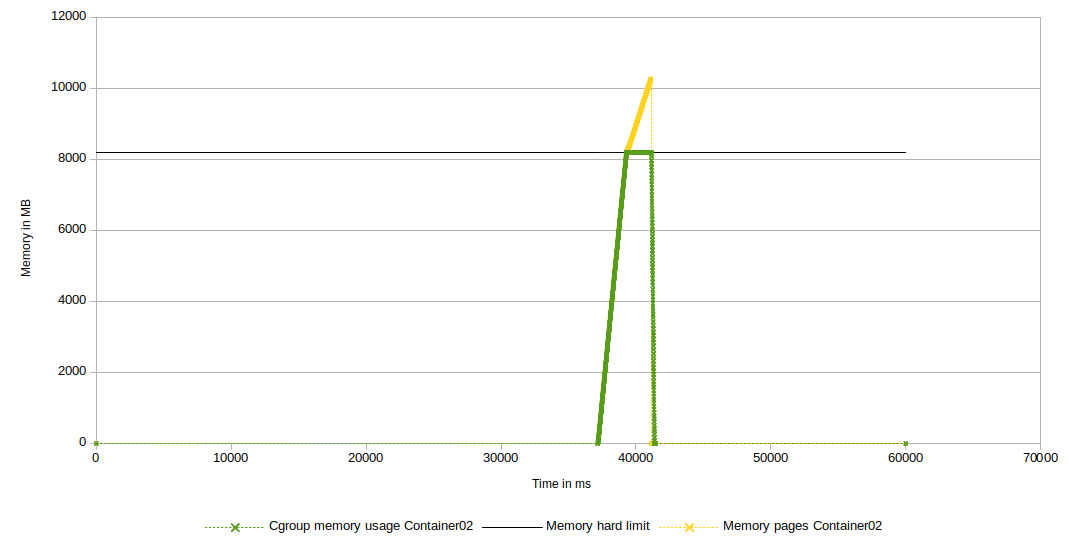
\includegraphics[width=1\linewidth]{pics/005_mem_usage_8200mb_limit_Container02_Basis_RDY_FOR_USE_FOCUS.png}
	\captionof{figure}[Speicher Verbrauch Cgroup 8200MB Limit]{Memory usage Cgroup 8200MB Limit}
	\label{fig:005_mem_usage_8200mb_limit_Container02_Basis_RDY_FOR_USE_FOCUS}
\end{minipage}

\subparagraph{Erwartungshaltung Test 05}
Die verwendbaren Systemressourcen liegen nach Abbildung \ref{fig:001_mem_usage_No_Limit_Cgroup_RDY_FOR_USE} bei etwa 14000MB. Allein Container01 verwendet schon ca. 8600MB der gesamten Summe, was die Deckelung bei Container02 auf 8200MB Wahrscheinlich unnötig macht, da dieser Wert mit den verwendbaren Ressourcen nicht erreicht werden kann. 

\vspace{1em}
\begin{minipage}{\linewidth}
	\centering
	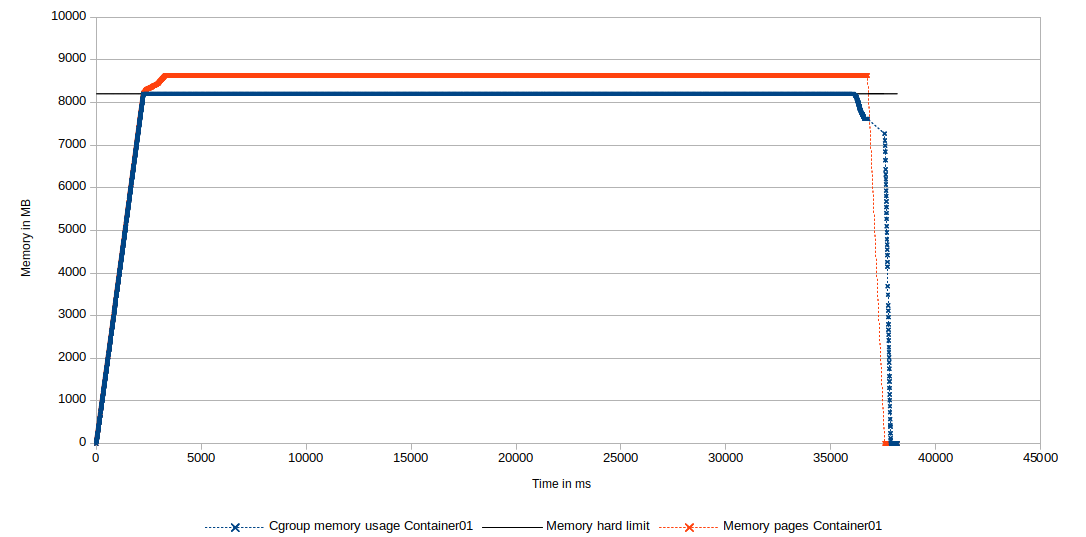
\includegraphics[width=1\linewidth]{pics/006_mem_usage_8200mb_limit_Container01_mit_ipact_RDY_FOR_USE.png}
	\captionof{figure}[Speicher Verbrauch Cgroup 8200MB Limit]{Memory usage Cgroup 8200MB Limit}
	\label{fig:006_mem_usage_8200mb_limit_Container01_mit_ipact_RDY_FOR_USE}
\end{minipage}

\subparagraph{Ergebnis Test05}
Nach Betrachtung von Abbildung \ref{fig:006_mem_usage_8200mb_limit_Container01_mit_ipact_RDY_FOR_USE} ist zu erkennen, dass Container01 nicht nach 60
\pagebreak
